\section{Data Construction for Cross-Game Learning}
\label{sec:data_construction}

Raw gameplay videos provide rich visual and control experience, but they rarely specify the player's objective, the decisions that require reasoning, or the information that should be retained beyond the recent context. We develop a scalable annotation pipeline that turns heterogeneous recordings into supervision for long-horizon task following, as shown in Figure~\ref{fig:data_construction}. Starting from tens of thousands of hours of raw gameplay collected across different sources, we filter invalid or misaligned recordings and balance coverage across gameplay scenarios. For SFT, we curate approximately 1K hours of gameplay trajectories. GPT-5.6-Luna~\cite{gpt56card} generates sparse action reasoning, task segments with instructions and scene descriptions, and task-state memories. We organize these annotations into three instruction levels: local operations, intermediate subgoals, and extended task stages.

\begin{figure*}[!htbp]
    \centering
    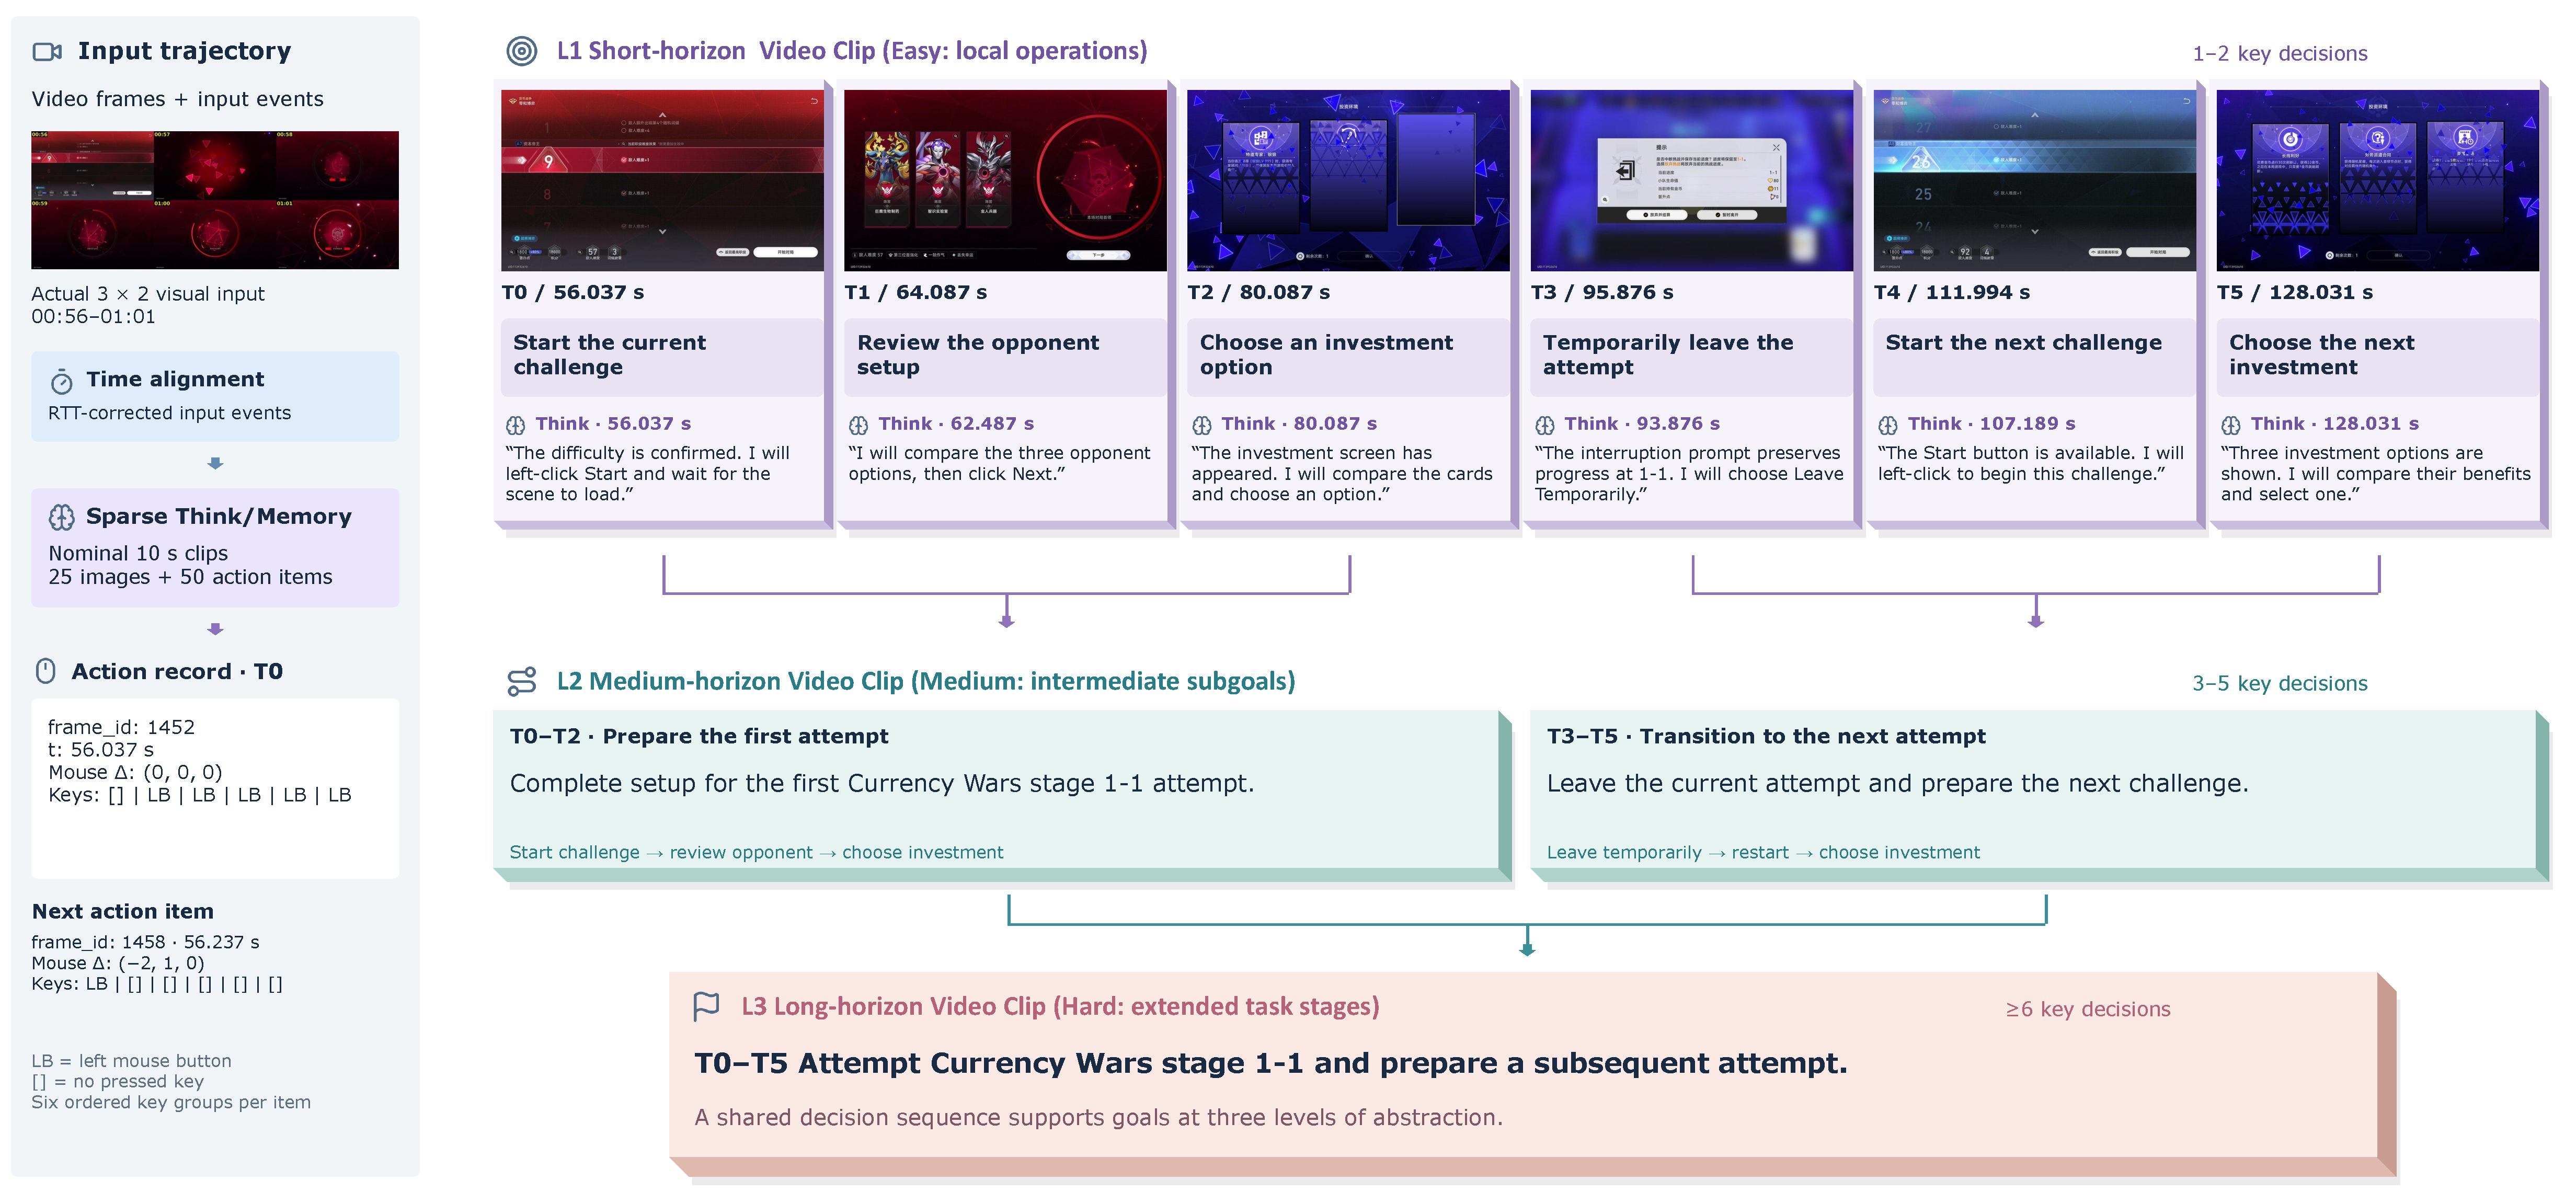
\includegraphics[width=0.92\linewidth]{figs/data_annotator.pdf}
    \caption{
    \textbf{Bottom-up construction of multi-level task supervision.}
    The diagram illustrates the organization of aligned gameplay segments into local operations, intermediate subgoals, and extended task stages. Separate GPT-5.6-Luna passes produce sparse Think annotations, segment-level instructions and scene descriptions, and memory updates as detailed in Secs.~\ref{sec:data_annotation}-\ref{sec:data_memory}. The diagram focuses on hierarchy assembly rather than depicting every annotation call.
    }
    \label{fig:data_construction}
\end{figure*}

\subsection{Trajectory Preparation and Temporal Alignment}
\label{sec:data_harmonization}

\textbf{Data sources, filtering, and scenario balancing.}
We collect raw gameplay recordings with associated keyboard and mouse events from multiple sources. Within this collection, the HSR recording track contains roughly 68K sessions and 11K hours of video. Rather than annotating all available videos, we first select recordings with reliable visual and action supervision. We reject corrupted or duplicated sessions, missing or discontinuous frames, and trajectories whose video and action timestamps cannot be aligned consistently. We also remove invalid action traces, including mouse coordinates outside the valid screen or control bounds, malformed action states, and events that cross recording or interaction boundaries. Long inactive periods and recordings without meaningful interaction are filtered, while valid held inputs and task-related waiting periods are retained.

Filtering alone would leave the instruction corpus dominated by frequently recorded activities. We therefore balance scenario coverage by limiting repeated behaviors and retaining less frequent interactions and longer task transitions. 
% This sampling step limits repeated or overrepresented behaviors while retaining examples of less frequent interactions and longer task transitions. It broadens the coverage of instruction supervision without requiring equal number of samples across categories. 
After these quality and coverage checks, we obtain \textbf{approximately 3.2K sessions and 1K hours of video}, which we use as the source for SFT annotation.

\textbf{Action-observation alignment.}
We retain the original ordering of keyboard and mouse events and associate each action block with its corresponding frame using corrected recording timestamps. Each device-level action interval spans approximately $200$ ms and contains the six finer control blocks defined in Sec.~\ref{sec:unified_action}. Source videos are sampled to obtain the visual observations used for annotation. When frame indices are discontinuous, or timestamps show a recording gap, an action window is not allowed to cross that boundary. Short button presses are kept as short pulses rather than being dropped by temporal aggregation. This preserves movement duration and interaction timing while producing the same executable action interface used by the policy. 

\subsection{Sparse Reasoning and Visual Task Segmentation}
\label{sec:data_annotation}

The annotation process separates local action reasoning from longer visual task understanding. Short video-action windows identify key decisions, while longer visual clips reveal task structure and progress. We use GPT-5.6-Luna for both annotation passes and align their outputs by the original frame IDs and recording timestamps. 
% The long-context pass uses visual mosaics only, without supplying the action JSON or the previously generated Think text.

\textbf{Decision-focused Thinking.}
We divide the action stream into windows of 50 device-level action intervals, corresponding to roughly 10 seconds of interaction. Each window contains 25 ordered game observations and the associated 50 action intervals. GPT-5.6-Luna identifies a sparse set of decision points, typically when the player selects or corrects a route, handles a new interaction prompt, changes objective, recovers from an unsuccessful attempt, or responds to a significant scene transition. Each \texttt{Think} annotation describes the observed outcome, the current decision, and an intended next action. Continuous movement, repeated controls, and minor camera corrections usually receive no separate reasoning target. Windows with neither meaningful input nor visual change can be skipped.
% while visually changing cutscenes remain eligible for annotation. 
% This process yields approximately \textbf{1.2M timestamp-aligned Think annotations}. These annotations are retrospective supervision tied to demonstrated behavior, rather than claims about the human player's private reasoning.
This process yields approximately \textbf{1.2M timestamp-aligned Think annotations}.

\textbf{Long-context instruction and scene annotation.}
% Unlike the earlier pipeline that produced a standalone caption for every sampled frame, the HSR pipeline derives a concise \texttt{scene} description together with each task segment. A session is divided into visual clips of at most 288 seconds. 
We divide each session into the minimum number of equal-length visual clips of at most 288 seconds.
Frames are selected at approximately one-second intervals and arranged into $3\times2$ timestamped mosaics, yielding at most 49 mosaic images per clip. This lets GPT-5.6-Luna inspect continuous visual context without exceeding the image-input budget. The model identifies contiguous task segments and assigns each a task \texttt{instruction}, a gameplay \texttt{label}, and a short \texttt{scene} description of the visible evidence. These task segments provide the temporal and semantic basis for the instruction hierarchy.

% We encourage activity segments to follow meaningful boundaries such as entering a game mode, completing a dialogue, restarting a challenge, or moving to a new task. Very short transitions are merged with adjacent activities, while separate attempts are kept distinct when the recording clearly shows a restart. Segment boundaries are checked for gaps and overlaps and are mapped back to absolute recording time. This yields approximately \textbf{63K activity segments}, with a median duration of about 40 seconds. The activity labels cover seven gameplay categories: navigation, NPC dialogue, combat, minigames, system menus, Currency Wars, and other activities.
We prompt the model to segment gameplay by the player's current task. Brief movements and reward collection are grouped with the task they support, while an explicit challenge restart begins a new segment. Postprocessing adjusts adjacent segment boundaries to form a continuous timeline and converts clip-relative start and end times to timestamps in the original recording. This yields approximately \textbf{63K task segments}, with a median duration of about 40 seconds. The activity labels cover seven gameplay categories: navigation, NPC dialogue, combat, minigames, system menus, Currency Wars, and other activities.

\subsection{Memory Annotation from Continuous Visual Context}
\label{sec:data_memory}

% A segment instruction describes the current objective but cannot preserve the state of a long task. We therefore generate compact memory annotations after the visual task segments have been identified. For each visual clip, the cleaned first-pass segments are returned to GPT-5.6-Luna as an assistant message in the same annotation conversation. A subsequent user message requests all memory windows in a single response, while the model retains the clip's earlier visual and task context. The windows are approximately 16 seconds long, with shorter tails merged when necessary. This preserves a shared visual and task context across successive memory updates within the clip. Each update contains a concise first-person \texttt{done} summary of what has happened by the end of its window. Its output records a start time, end time, and \texttt{done}. The active instruction and an associated frame ID are added during postprocessing. A failed attempt is recorded only after its failure becomes observable.
After task segmentation, we reuse the clip images and cleaned task segments in a second conversational turn to generate memory annotations. The model returns all summaries for the clip in one response, typically one per 16-second window. Each summary briefly describes, in the first person, the cumulative accomplishments and outcomes within the clip up to the window end. A final window shorter than 8 seconds is merged into the preceding window. Postprocessing associates each summary with the active task instruction and the latest image frame at or before the window end.

% The resulting dataset contains approximately \textbf{223K memory annotations}, each indexed by its start and end timestamps and associated with an active instruction. In the training phase, a summary is selected only when its end timestamp is no later than the current observation, so that it cannot be introduced before its stated availability. The memory therefore represents completed task state rather than another frame caption. Consecutive summaries track progress within each visual clip. Longer task dependencies are represented through the memory interface used by SFT. The annotation prompt restricts each memory to events observable by its timestamp, and training presents a summary only after its associated window ends. Because annotation uses the complete visual clip, this causal constraint is enforced at the instruction and timestamp-selection levels rather than through per-window visual masking. For example, a challenge segment may remain unresolved in one memory window and be marked as failed only after a later window shows the result and the start of another attempt.
The dataset contains approximately \textbf{223K memory annotations}. At each training step, we condition the policy on the latest summary whose end timestamp is no later than the current observation. The annotation model receives the complete visual clip and is prompted to summarize only events up to each window end.

\subsection{Three-Level Instruction Construction}
\label{sec:multi-level_supervision}

% The first-pass activity segments provide grounded objectives, but they do not alone supply all the temporal horizons needed for long-horizon instruction following. We therefore build three \textbf{instruction-granularity levels} over the second-generation HSR annotations, following the easy, medium, and hard organization used in our earlier construction. These levels should not be confused with the seven gameplay categories or interpreted as measured difficulty for human players. They reflect how many decision points and local objectives must be coordinated within an instruction. The three levels may cover overlapping portions of the same original recording.
Building on the first-pass task segments, we construct \textbf{easy, medium, and hard instructions} according to the scope of the objective and the number of annotated decisions it covers. These levels correspond to local operations, intermediate subgoals, and extended task stages, respectively. The same recorded interval can support instructions at multiple levels.

\textbf{Easy: local operations.}
Easy instructions cover one or two annotated decisions, such as approaching an NPC, selecting a menu option, or collecting an item. \textbf{Medium: intermediate subgoals.} Medium instructions combine related operations into a subgoal spanning three to five annotated decisions, such as navigating around an obstruction and completing the required interaction. \textbf{Hard: extended task stages.} Hard instructions connect multiple subgoals into a task stage spanning six or more annotated decisions, such as navigating through several areas and resolving intervening challenges.

% We construct these views bottom-up from temporally aligned annotations. The activity-level instructions and scene evidence establish what the recorded player actually does. Sparse Think annotations identify important transitions, while memory records the evolving task state. Human-annotated examples guide the intended wording and scope of generated instructions. Adjacent, compatible operations can be grouped into subgoals and then extended task stages. Across the three levels, the \textbf{original action sequence and its accepted Think annotations are not regenerated}. Only the instruction context and the memory horizon change. The retained supervision thus teaches one policy to execute the same actions under progressively longer objectives rather than creating synthetic action trajectories.
We construct the instruction hierarchy bottom-up from temporally aligned annotations. Task-segment instructions and scene descriptions establish the activity and its boundaries, Think annotations identify key decisions, and memories track task progress. We group adjacent operations that advance a common subgoal, then combine related subgoals into extended task stages. Human-annotated examples guide the wording and scope of the generated instructions. All three levels share the \textbf{recorded actions and Think annotations}, and each provides an instruction and memory context appropriate to its objective.

\textbf{Horizon-dependent training targets.}
For a selected supervision horizon $h\in\{\mathrm{op},\mathrm{sub},\mathrm{task}\}$, an example is represented as
\begin{equation}
    x_t^{h}=\left(\mathcal{B},I^{h},\mathcal{M}_t^{h},\mathcal{H}_t\right),
    \qquad y_t=[r_t,a_t],
    \label{eq:multi-level_supervision}
\end{equation}
% where $I^{h}$ denotes the current instruction and $\mathcal{M}_t^{h}$ the memory associated with that horizon. Recent history $\mathcal{H}_t$, sparse reasoning $r_t$, and executable action $a_t$ are grounded in the same recorded trajectory. An action target is present at every step, including steps without explicit Think annotation. Operation-level examples emphasize local control, medium examples require coordination across several interactions, and hard examples demand more persistent task state. This links the data pipeline directly to the sparse reasoning and memory mechanisms learned during SFT.
where $I^{h}$ denotes the task instruction at level $h$, $\mathcal{M}_t^{h}$ denotes its task memory, and $\mathcal{H}_t$ contains the current observation and recent interaction history. The reasoning text $r_t$ and action target $a_t$ are drawn from the same recorded trajectory and its annotations. Every step includes action supervision, including steps without Think annotations.

 Unlike GameHorizon\cite{wang2026gamehorizon}, \ourmodel builds high level instruction data from aligned gameplay videos and actions uses a separate annotation passes to identify task boundaries and label decision points. The first pass identifies task boundaries within visual clips. The second examines short video-action windows and adds sparse \texttt{Think} annotations at decision points (Sec.~\ref{sec:data_annotation}). Each training example provides supervision for keyboard and mouse actions at every step and for reasoning at selected decision points. Timestamped summaries supply context on task progress (Sec.~\ref{sec:data_memory}).


% \textbf{Quality control and data consistency.}
% We apply structural and temporal consistency checks to improve the quality of annotated trajectories. Specifically, we resolve gaps and overlaps between task segments, merge activity segments shorter than 16 seconds, and align reasoning and memory annotations with the original interaction timeline. Instructions and scene descriptions are grounded in recorded observations, while memory annotations are constrained to reflect the task state available at each step. We further construct easy, medium, and hard supervision from the same underlying trajectories, providing different instruction and memory horizons while preserving the original executable actions.


